\documentclass[fleqn]{article}

\usepackage{polski}
\usepackage[utf8]{inputenc}
\usepackage[polish]{babel}
\usepackage{parskip}
\usepackage{icomma}
\usepackage[a4paper,includeheadfoot,margin=1.27cm]{geometry}
\usepackage{float}
\usepackage{graphicx}
\usepackage{amsmath}
\usepackage[hypcap=true]{subcaption}
\usepackage{xcolor}
\usepackage{transparent}
\usepackage{listings}
\usepackage[colorlinks=true, linkcolor=blue, pdfborder={0 0 0}]{hyperref}

\renewcommand\thesection{\arabic{section}.}
\renewcommand\thesubsection{\alph{subsection})}
\renewcommand\thesubsubsection{}
\newcommand\square[1]{
	\fcolorbox{black}{#1}{\rule{0pt}{6pt}\rule{6pt}{0pt}}
}

\brokenpenalty=1000
\clubpenalty=1000
\widowpenalty=1000

\title{TM -- Laboratorium 3. \\ \large Licznik 8-bitowy – zerowanie, zliczanie w górę do zadanej wartości – kod NKB}
\author{Krystian Chachuła \\ Dawid Gruszczyński \\ Marcin Skrzypkowski}

\begin{document}

\maketitle

\setcounter{page}{0}
\thispagestyle{empty}

\pagebreak

\setcounter{page}{1}

\section{Wstęp}

Na trzecim laboratorium mieliśmy za zadanie, korzystając z modułu mikrokontrolera MSP430 oraz innych modułów SML-3, zaprojektować i zrealizować licznik zliczający w górę w kodzie NKB z możliwością asynchronicznego zerowania jego zawartości.
Sterowanie licznikiem miało odbywać się za pomocą dwóch przycisków (CLK aktywne zboczem oraz CLR aktywne poziomem).
Dodatkowym wymogiem zadania była realizacja programowej eliminacji drgań styków oraz obsługa przynajmniej jednego z przycisków z użyciem przerwań oraz ograniczanie maksymalnej wartości licznika z pomocą przełączników szesnastkowych.

Zaprojektowany przed laboratorium układ zbudowaliśmy z następujących układów SML-3:

\begin{itemize}
	\item \textbf{10\_PS1} (moduł zasilacza)
	\item \textbf{160\_7SEG2} (moduł wyświetlacza 7 segmentowego)
	\item \textbf{120\_IN8} (zestaw 8 monostabilnych wyłączników)
	\item \textbf{451\_IN\_4xHEX} (moduł przełączników szesnastkowych)
	\item \textbf{570\_MSP430F14x} (moduł mikrokontrolera Texas Instruments serii MSP430f14x lub F16x)
\end{itemize}

\section{Implementacja licznika}

Projektowanie rozpoczęliśmy od stworzenia grafu stanów, który przedstawiał ogólny schemat działania licznika.
%TODO ogarnąć grafuu

\begin{figure}[H]
	\centering
	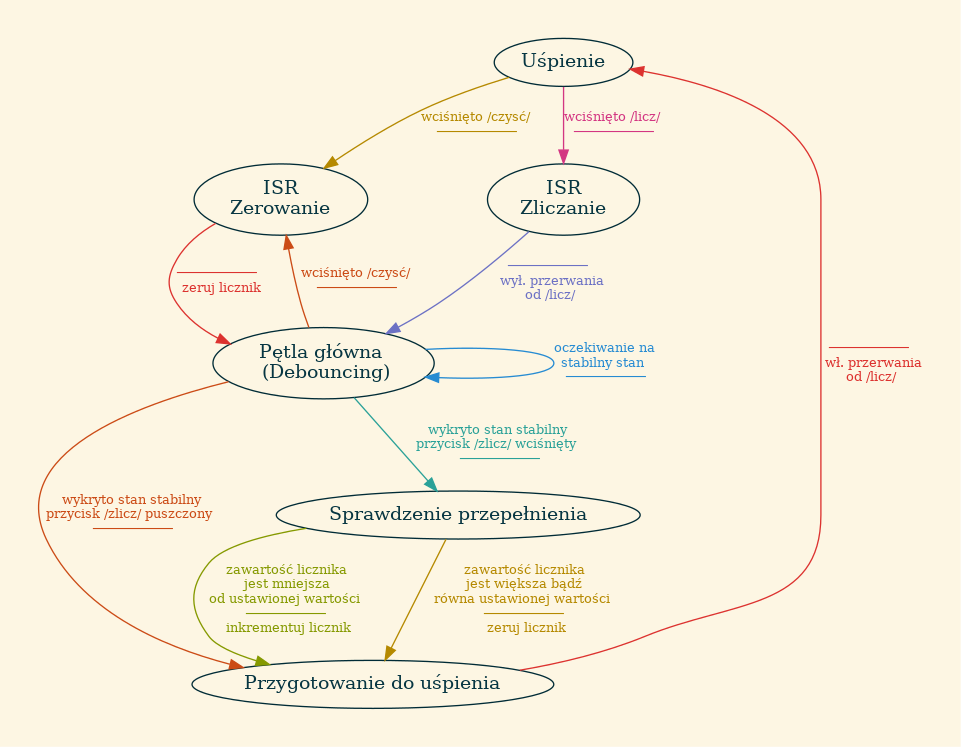
\includegraphics[width=\textwidth]{assets/graph.png}
	\caption{Graf automatu stanów}
	\label{fig:graph}
\end{figure}


Na początku pracy, mikrokontroler znajduje się w stanie uśpienia. Wybudzenie następuje tylko w przypadku wystąpienia przerwania z portu P1 (zbocze przycisku CLR) lub portu P2 (zbocze przycisku CLK). Następnie następuje przejście do obsługi zgłoszonego przerwania.

W przypadku przerwania od przycisku CLK, wyłączane są tylko przerwania generowane przez ten przycisk oraz trwale wybudzany jest mikrokontroler (przejście do pętli głównej programu). W przypadku przerwania od przycisku CLR zerowane jest wyjście licznika, zerowana jest zawartość rejestru służącego do usuwania drgań styków (rejestr R5) oraz wyłączane są przerwania od przycisku CLK (na czas trzymania wciśniętego przycisku CLR nie chcemy by istniała możliwość wywołania przerwania zliczającego). Wybudzany jest także trwale mikrokontroler.

Przerwania zliczające mogą być wywoływane tylko w momencie gdy mikrokontroler jest w stanie uśpienia, natomiast przerwania zerujące mogą być wywoływane w każdym miejscu poza sekcją krytyczną związaną z inkrementacją licznika. Przerwania nie mogą być zagnieżdżane. W pętli głównej programu, sprawdzane jest czy wciśnięty jest przycisk zerujący (w przypadku zerowania licznika blokujemy możliwość inkrementacji do momentu puszczenia przycisku CLR) oraz czy wciśnięty jest przycisk zliczania (eliminacja drgań w przypadku inkrementacji licznika).

Eliminacja drgań przy wciśnięciu przycisku odbywa się w następujący sposób. Z każdym obiegiem pętli sprawdzany jest stan na pinie do którego podłączony został przycisk CLK. Ilość obiegów, a zatem ilość próbek zawarta jest w rejestrze R7. Liczba ta określa czas przez jaki sprawdzane jest występowanie drgań styków przycisku. Jeżeli przy sprawdzaniu na pinie panuje stan niski (wciśnięty przycisk), inkrementowany jest rejestr R5, w przeciwnym przypadku inkrementacja jest pomijana. W momencie gdy sprawdzanie jest zakończone, sprawdzana jest zawartość rejestru R5. Jeżeli jest ona równa zawartości rejetru R7 oznacza to, że przycisk jest stabilnie wciśnięty a więc następuje inkrementacja licznika. Jeżeli jest ona równa zero oznacza to, że przycisk został puszczony, a więc zakańczana jest pętla główna a procesor zostaje ponownie uśpiony. W pozostałych przypadkach podejmowana jest kolejna próba sprawdzania drgań, ponieważ stan na pinie nie jest stabilny.

W trakcie inkrementacji licznika ustawiana jest flaga informująca o tym, że licznik został zinkrementowany, dzięki czemu możliwa jest eliminacja drgań przy puszczeniu przycisku w taki sam sposób jak przy wciśnięciu (po zanotowaniu stabilnego wciśnięcia licznik nie będzie inkrementowany dzięki warunkowi sprawdzającemu tę flagę). Stan przycisku sprawdzany jest aż do momentu wykrycia stabilnego stanu wysokiego na pinie informującego o puszczeniu przycisku.

Proces eliminacji drgań może zostać przerwany przez wciśnięcie przycisku CLR, w takim przypadku licznik jest zerowany, a jego inkrementacja nie następuje nawet w przypadku gdy przycisk CLK jest wciśnięty. Po zakończeniu zerowania lub inkrementacji licznika, zerowane są odpowiednie rejestry oraz włączane są przerwania przycisku zliczającego, następnie mikrokontroler ponownie jest usypiany.

Na podstawie grafu powstał kod napisany w języku Assembly.



\section{Kod programu oraz jego opis}

\subsection{Blok Init}
		Na samym początku programu ustawiany jest wskaźnik stosu i wyłączany niepotrzebny w naszym obecnym projekcie watchdog, który nieobsłużony powodowałby niepożądany reset mikrokontrolera.
		W bloku \textit{Init} następuje ustawienie podstawowych flag przed rozpoczęciem działania licznika, a więc:
		\begin{itemize}
			\item następuje przypisanie przycisków zliczania i resetu do odpowiednich linii portów
			\item następuje odblokowanie przerwań pinów, do których są podłączone przyciski
			\item następuje wyzerowanie rejestru do debouncingu (\textit{R5}) oraz rejestru przechowującego pomocniczą flagę przerwania zerującego (\textit{R6})
			\item skonfigurowanie odpowiednich portów
		\end{itemize}

		W następnym bloku procesor od razu jest wprowadzany w stan oszczędzania energii LPM4 (wyłączone wszystkie zegary i procesor), z którego może być wybudzony tylko przerwaniem przycisku CLK bądź CLR. Po wybudzeniu następuje przejście do głównej części pętli.

\subsection{Procedura loop\_1}
		Pierwszą instrukcją, jaka jest wykonywana w tej procedurze, jest sprawdzenie wciśnięcia przycisku resetu. Jeśli jest on wciśnięty, następuje zapętlenie do loop\_1. Jeśli nie jest oznacza to, że albo został on właśnie puszczony, albo nie wystąpiło przerwanie zerujące a mikropocesor jest w trakcie sprawdzania dgrań przycisku zliczającego. W celu kontunuacji sprawdzana jest pomocnicza flaga znajdująca się w rejestrze R6, która ustawiana jest gdy wywoływane jest przerwanie zerujące. W sytuacji gdy jest ona równa 0, mikrokontroler może kontynuwać pracę, w przeciwnym przypadku następuje skok do procedury \textit{loop\_3} zakańczającej główną pętlę. Następnie, w celu eliminacji drgań styków, sprawdzany jest stan przycisku zliczającego. W przypadku gdy jest on wciśnięty następuje inkrementacja zawartości rejestru R5, w przeciwnym razie jest ona pomijana. Przy każdym obiegu sprawdzającym stan przycisku inkrementrowana jest także zawartość rejestru R7 (rejestr ten mówi o tym ile obiegów pętli zostało wykonanych). W momencie gdy zawartość tego rejestru równa jest stałej wartości \textit{DEB\_TIME}, informującej o ilości obiegów pętli jakie należy wykonać w celu poprawnej eleminacji dgrań, następuje sprawdzenie czy w momencie próbkowaniu stanu przycisku na pinie panował stan stabilny. W tym celu zawartość rejestru R5 porównywana jest z zerem oraz z wartością przechowywaną w rejestrze R7. W momencie gdy w rejestrze tym znajduje się 0 (brak drgań, stabilny stan wysoki - przycisk nie jest wciśnięty), następuje skok do procedury \textit{loop\_3} zakańczającej pętlę główną i usypiającej procesor, natomiast gdy zawartość rejestru równa jest zawartości rejestru R7 (brak drgań, stabilny stan niski - przycisk jest wciśnięty) następuje skok do procedury \textit{main\_inc} (inkrementacja licznika). Jeżeli żadna z tych wartości nie znajduje się w rejestrze oznacza to, że stan na pinie nie jest stabilny, a więc proces sprawdzania drgań jest ponawiany.

\subsection{Procedura main\_in}
		Na początku bloku inkrementacji sprawdzana jest flaga mówiąca o tym, czy licznik był wcześniej inkrementowany. W przypadku gdy jest ona równa 1, następuje przejście do procedury \textit{loop\_1}. Jeżeli flaga ta jest róna równa 0, zostaje ona ustawiona. Następnie zawartość licznika porównywana jest z wartością ustawioną na przełącznikach szesnastkowych. Jeżeli wartość na przełącznikach jest równa bądź mniejsza niż aktualna wartość licznika głównego, jest on resetowany, w przeciwnym przypadku następuje inkremetacja licznika. W obu sytuacjach następuje przejście do procedury \textit{loop\_1}.

\subsection{Procedura loop\_3}
		W tej procedurze następuje czyszczenie rejestrów używanych do debouncingu i reset flag przerwania oraz pomocniczych. Następnie odblokowane zostają przerwania od CLK i następuje powrót do stanu oszczędzania energii.

\subsection{Blok Przerwań}
		Po wystąpieniu przerwania od przycisku zliczania resetowane są bity odpowiedzialne za wprowadzanie mikrokontrolera w stan oszczędzania energii, aby procesor mógł przejść po jego obsłudze do pętli głównej. Blokowane są również przerwania od tego przycisku, aby podczas sprawdzania drgań nie były zgłaszane kolejne przerwania zliczające. Po powrocie z przerwania następuje przejście do procedury \textit{loop\_1}.

		Po wystąpieniu przerwania resetującego resetowany jest licznik główny, resetowane są flagi przerwań obu przycisków, aby po wyjściu z przerwania nie zgłaszały one przerwań, oraz wyłączane są przerwania zliczające, aby nie mogły być one wywoływane po wyjściu z obsługi przerwania resetującego (podczas gdy przycisk CLR jest wciśnięty nie chcemy by istaniła możliwość wywołania przerwania od przycisku CLK). Następnie resetujemy rejestr odpowiedzialny za eliminację drgań i ustawiana jest pomocnicza flaga oznajmiająca wystąpienie przerwania resetującego (zerowy bit rejestru \textit{R6}) i podobnie jak w przerwaniu przycisku zliczającego trwale wybudzamy mikrokontroler, by znowu móc pracować z pełną mocą. xD

\subsection{Sekcja krytyczna}
		Blok sekcji krytycznej występuje w okolicach inkrementacji licznika głównego. Jest ona konieczna, powieważ w przypadku gdyby zaraz po zakończeniu debouncingu nastąpiło przerwanie od przycisku CLR, rejestr \textit{R5} i licznik główny zostałyby zresetowane, lecz zaraz po zakończeniu obsługi przerwania licznik byłby inkrementowany.

		Wyłączanie przerwań jest konieczne również w trakcie wchodzenia do procedury \textit{loop\_3} oraz jej wykonywania. Wywołanie przerwania CLR w trakcie jej wykonywania, co prawda powodowałoby zerowanie licznika, lecz zaraz po nim procesor lądowałby w stanie uśpienia z włączonymi przerwaniami zliczającymi i mimo, że przycisk byłby nadal wciśnięty, istniałaby możliwość inkrementacji licznika. Dodatkowo zgłoszenie przerwania przycisku zliczającego zaraz po aktywacji jego przerwań powodowałaby blokowanie możliwości inkrementacji licznika (w trakcie obsługi przerwania zliczającego, przerwania te są trwale wyłączane) - procesor byłby usypiany z wyłączonymi przerwaniami zliczającymi.


\textbf{Kod programu:}

\lstinputlisting{src/main.asm}





\section{Podłączenie procesora}

Przyciski sterujące pracą licznika podłaczyliśmy do portów P1 oraz P2, (przycisk CLR do pinu 1 portu P1, ponieważ musi on posiadać większy priorytet, natomiast przycisk CLK do pinu 4 portu P2). Wyjściem licznika jest port P3 skonfigurowany jako wyjście, którego zawartość wyświetlana jest za pomocą modułu wyświetlacza 7 segmentowego. Do wczytywania wartości zadanej, do której ma zliczać licznik, wykorzystaliśmy port P4 skonfigurowany jako wejście. Jest on bezpośrednio podłaczony do modułu przełączników szesnatkowych.

\section{Możliwości rozwoju}

Możliwym udoskonaleniem zadania byłoby dodatkowe sprawdzanie poprawności odczytu wartości zadanej z modułu przełączników szesnastkowych. Odczyt w złym momencie może powodować przekłamania niektórych bitów spowodowane przełączaniem między pozycjami. Aby mieć pewność, że odczytany stan jest stabilny, należy kilkukrotnie odczytać sygnał wejściowy na porcie P4 i sprawdzić, czy odczytane wartości nie rożnią się między sobą. W przypadku różnic należy przeprowadzać ponowne odczyty aż do momentu uzyskania wartości stabilnej.

\end{document}
\grid
